\section{子问题二：月度充电成本预测}

\subsection{问题定义与难点}

任务二的目标是预测用户每月的充电总支出 monthly\_charging\_cost，金融机构可据此评估用户的用车经济压力。题面建议的输入特征包括 electricity\_cost\_per\_kwh、monthly\_energy\_consumption\_kwh（可用任务一的预测值作为级联特征）、fuel\_expense\_per\_month 等，并提示该问题``高度非线性''。

数据探索阶段的关键发现是：充电成本几乎等于月能耗与电价的乘积（$R^2=0.9994$）。因此本任务的难点并不在于拟合复杂的非线性关系，而在于如何在没有真实能耗的情况下，以无泄漏的方式构造级联预测。

\subsection{核心物理关系}

如图\ref{fig:t2_scatter}所示，monthly\_charging\_cost 与 ``monthly\_energy\_consumption\_kwh $\times$ electricity\_cost\_per\_kwh'' 几乎严格落在对角线 $y=x$ 上，全量数据拟合 $R^2=0.9994$、RMSE=0.60。这意味着充电成本由一个确定性公式刻画，唯一的建模空间在于能耗的预测精度。

\begin{figure}[H]
\centering
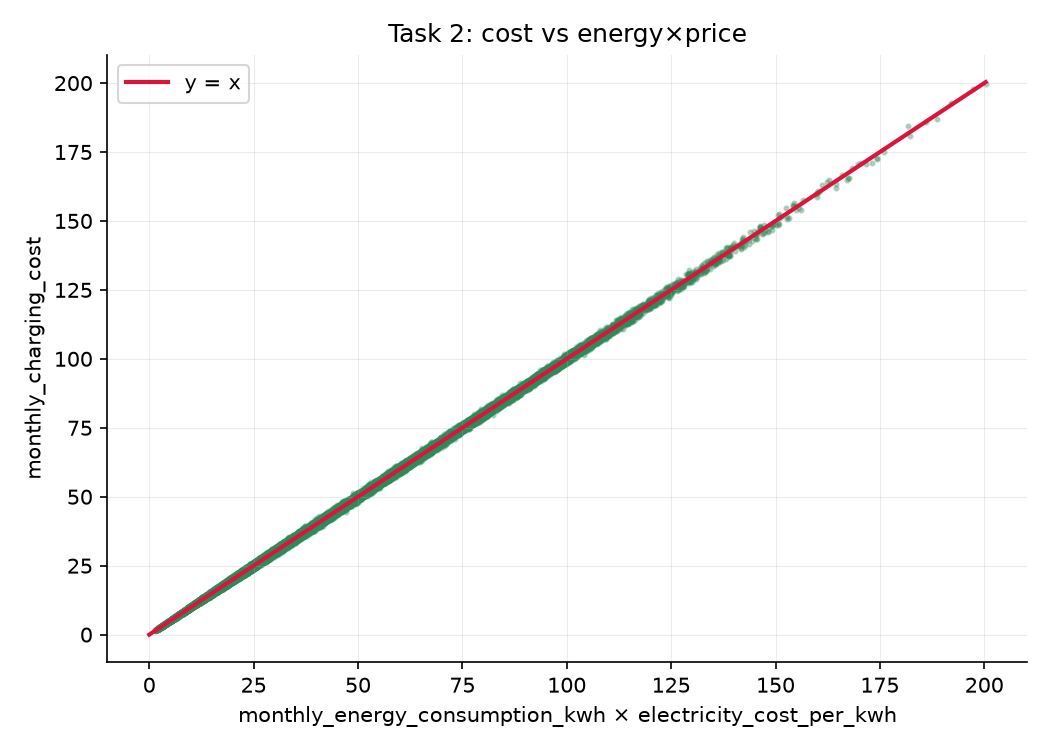
\includegraphics[width=0.8\textwidth]{figures/task2_cost_scatter.png}
\caption{充电成本与能耗$\times$电价的关系}
\label{fig:t2_scatter}
\end{figure}

\subsection{泄露边界与严格嵌套级联}

任务二的关键风险在于\textbf{teacher forcing}：如果在训练时使用真实能耗、而在测试时改用任务一的预测能耗，将造成训练与推理的分布错位，线下指标虚高而线上崩溃。为规避这一风险，本文设计了严格嵌套 OOF 级联方案：

\begin{enumerate}[itemsep=0pt]
\item 划分任务二的外层训练折 $A$ 与验证折 $B$；
\item 在 $A$ 内部再次交叉验证任务一，为 $A$ 中每行生成内层 OOF 能耗预测；
\item 用 $A$ 的全部数据重训任务一模型，预测 $B$ 的能耗；
\item 在 $A$ 上使用内层 OOF 能耗、在 $B$ 上使用外层预测能耗，分别构造 $\hat{cost} = \hat{energy} \times price$；
\item 汇总所有外层 $B$ 得到任务二的最终 OOF 预测。
\end{enumerate}

该方案从机制上保证了验证折的能耗预测从未见到验证折的真实能耗，杜绝了跨折信息传递。

\subsection{实验结果}

\subsubsection{方案对比}

任务二的各方案对比如表\ref{tab:t2_results}所示。

\begin{table}[H]
\centering
\caption{任务二方案对比（5 折 OOF）}
\label{tab:t2_results}
\begin{tabular}{lccc}
\toprule
\textbf{方案} & \textbf{$R^2$} & \textbf{adj-$R^2$} & \textbf{说明} \\
\midrule
严格嵌套级联（$\hat{energy}\times price$） & \textbf{0.917824} & \textbf{0.917820} & 主方案 \\
无级联 Ridge（周里程+日通勤+电价） & 0.851358 & 0.851349 & 对比基线 \\
真实能耗 $\times$ 电价 & 0.999428 & 0.999428 & Oracle 上界 \\
\bottomrule
\end{tabular}
\end{table}

严格嵌套级联方案得到 adj-$R^2=0.917820$，显著优于不依赖级联的对比基线（0.851358）。Oracle 方案（0.999428）说明，若测试时提供真实能耗，理论上界接近 1；但该值仅作诊断参照，不参与排名。

\subsubsection{级联后的进一步建模}

本文进一步检验：在级联特征 $\hat{cost} = \hat{energy} \times price$ 之上做线性校准、或加入官方建议的燃油支出特征，能否带来增益。结果如表\ref{tab:t2_ablation}所示，两种做法均使 adj-$R^2$ 略有下降。

\begin{table}[H]
\centering
\caption{任务二级联后消融（adj-$R^2$）}
\label{tab:t2_ablation}
\begin{tabular}{lcc}
\toprule
\textbf{方案} & \textbf{特征数} & \textbf{adj-$R^2$} \\
\midrule
纯级联 $\hat{cost}$ & 2 & \textbf{0.917820} \\
级联 + 线性校准 & 3 & 0.917794 \\
级联 + 燃油支出特征 & 4 & 0.917791 \\
\bottomrule
\end{tabular}
\end{table}

这一结果表明，任务二的误差几乎全部来自任务一能耗预测的个体能效误差，而非成本映射本身；在级联之上叠加任何模型都只是增加自由度惩罚。

\subsection{最终模型}

任务二的最终模型为：

\begin{equation}
\hat{y}_2 = r_1 \cdot weekly\_travel\_distance\_km \cdot electricity\_cost\_per\_kwh
\label{eq:t2}
\end{equation}

其中 $r_1=0.8163487$ 复用任务一的比率系数。在 5 折 $\times$ 3 种子最终确认中，adj-$R^2$ 均值为 0.917817 $\pm$ 0.000004。
